% Chapter 5
\chapter{Evaluation}
% Step back and say things like:
% "X worked out well"
% "in hindsight we could have used this tool instead"

% How do we know that our code works?
% e.g. functionality + performance testing
% show relevant testing *results*

% In a nutshell, how successful was this project
% Tony: "DONT SAY: all our objectives (from intro) were met. Have the maturity
% to show your mistakes and more importantly what you learned!"


\section{Implementation}
% In here, we can evaluate our implementation ... Talk about why Haskell was slow for computing the experiments, how we overcame this, ...

\hilight{we need to add some sub-sections here, or bullet points ... this wall of text would only appeal to Chatley}
%why Haskell?
In a nutshell, we are content with the choice of our tools and with our implementation of the neural network. Since our mathematical core of the algorithm does not contain much state information, we chose to implement our project in Haskell.
The strong types allowed us to have confidence in the code we write. Since most of our experiments took a lot of computation time, we had to make sure they run seamlessly and don't crash in the middle of the execution because of a pattern match failure.

There are a lot of advantages in using Haskell, including its clarity and correctness. The type system enforces the programmer to have a clear understanding of the problem and the various solutions available, which leads to high quality code.
Using Haskell came with an initial price: while all the group members were familiar with the language due to our course in first year, we soon realised that we only played with Haskell before. Because of our project, we now deeply appreciate its true beauty and power.

This early overhead turned out to be very small compared to the benefits and the satisfactions we got back. The project enabled us to learn about neural networks and attachment types, but we chose to exploit this opportunity in order to become better using a programming language we like (see fig ~\ref{fig:Haskell Proficieny Index over time}).
\begin{figure}[h]
  \centering1
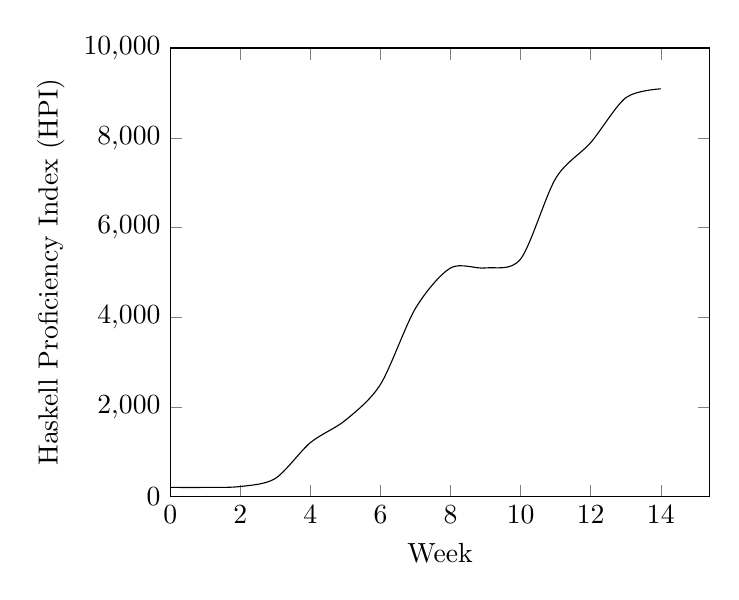
\begin{tikzpicture}
\begin{axis}[
xmin = 0,
ymin = 0,
xlabel = Week,
ylabel = Haskell Proficiency Index (HPI),
scaled y ticks = false,
y tick label style={/pgf/number format/fixed}
]

\addplot [
color = black,
mark = *, % A filled circle
mark = none,
smooth  % draw smooth curve
] coordinates {
(0,200)
(1,200)
(2,220)
(3,400)
(4,1200)
(5,1700)
(6,2500)
(7,4200)
(8,5100)
(9,5100)
(10,5300)
(11,7100)
(12,7900)
(13,8900)
(14,9100)
};

\end{axis}
\end{tikzpicture}

\caption{Average Haskell Proficiency Index over time.}
\label{fig:Haskell Proficieny Index over time}
\end{figure}

\subsection{Optimising for speed}

While testing the recognition application, we realised that our implementation was not as fast as we would have liked it to be, and imposed serious limitation on the size of the networks we were able to try out.
As a consequence, we invested a good amount of time in understanding Haskell compiler optimisations, runtime characteristics, and profiling tools. Using time and allocation profiling, we found that two inner loops in our numerical network updating code were slowing us down significantly. By changing 12 lines to manually unroll the involved list comprehensions into tail-recursive functions we were able to get an overall 4-times speedup of our program.
Additionally, Haskell's being a purely functional programming language allows for easy and efficient parallelism.
By replacing a top-level map with a parallel map function, our program immediately scaled up to the eight processes that were available on the lab machines we used. Because our main processing time is spent in numerical, cache-local loops, we also got almost 8-times improved performance from this. This final scaling success is an improvement over an initial try in which we parallelized an inner loop, which turned out to be too fine-grained.

% already good performance that we achieved through writing code without side effects and ghc's highly optimizing native code generator.

\subsection{Unit Testing}

Unit testing of our Haskell functions was performed using the HUnit framework. This allowed us to heavily test the complex functions responsible for performing updates or calculating energy and capacity, thus making sure that important invariants always hold: energy is always monotonically decreasing, capacity is following the theoretical trends and updates eventually converge to an attractor.

%show some testing results here

\section{Evaluating our deliverables}
% We can use this section to evaluate some of our experiments, point out any inconsistencies, limitations, ...

Our main task was twofold:

\begin{enumerate}
\item Implement the Hopfield model and a basic image recognition application to show its functionality.
\item Support or reject Federico's claims about clustering and evaluate his results in the context of Attachment Types.
\end{enumerate}

We implemented both of these goals: We have a clear, concise Haskell implementation of the Hopfield model with a public and well-tested API to train Hopfield networks and converge patterns in them. To show that it works in the real world, we built a police-style suspect face matching application with an accessible GUI, which in addition to performing image recognition also has a functionality to introduce a layman to how Hopfield networks work using interactive examples.

We implemented Federicos clustering experiments and checked the majority of his claims; as described in the analysis above, our independent results largely support his claims.

Extending our initial goals, we additionaly evaluated the influence of Super Attractors and their relation to Attachment Theory; we can conclude that Federicos results concerning clustering and our results concerning Super Attractors support the idea that Hopfield networks are a good way to model the real world domain of Attachement Types.

[BOLZMANN]

Finally, we came up with some our own way to use the Boltzmann machine for pattern matching, implemented the Storkey method as an alternative to Hebbian learning for increased network capacity, and proved properties about [...].
